\documentclass[a4paper,12pt]{article}
\usepackage[left=1.5cm,right=1.5cm,
    top=1cm,bottom=1.5cm,bindingoffset=0cm]{geometry}

\usepackage[T1,T2A]{fontenc}
\usepackage[utf8]{inputenc}
\usepackage[english,russian,ukrainian]{babel}
\usepackage{tabularx}
\usepackage{amssymb}
\usepackage{color}
\usepackage{amsmath}
\usepackage{mathrsfs}
\usepackage{listings}
\usepackage{graphicx}
\graphicspath{ {./images/} }
%\usepackage{draftwatermark} не будет лезть на картинки
\usepackage[printwatermark]{xwatermark}%будет лезть на картинки
\usepackage{lipsum}
\usepackage{xcolor}
\usepackage{tikz}
\newsavebox\mybox
\savebox\mybox{\tikz[color=red,opacity=0.07]\node{A n M n};}
\newwatermark*[
  allpages,
  angle=45,
  scale=11,
  xpos=-40,
  ypos=55
]{\usebox\mybox}
\definecolor{lgreen}{rgb}{0.5,1,1}
\definecolor{n}{rgb}{1,0.5,0.5}
\definecolor{n1}{rgb}{1,1,0.5}
\definecolor{n3}{rgb}{1,0.7,0.9}




\begin{document}
\pagecolor{white}
\large



В собственном полупроводнике свободные носители возникают только за счёт разрыва валентных связей, поэтому число дырок = числус вободных электронов, т.е. $n= \rho$ = $n_i$, где $n_i$ – собственная концентрация. Электропроводность:
\begin{center}
$\sigma = e\cdot n \cdot \mu_n + e\cdot p \cdot \mu_p$
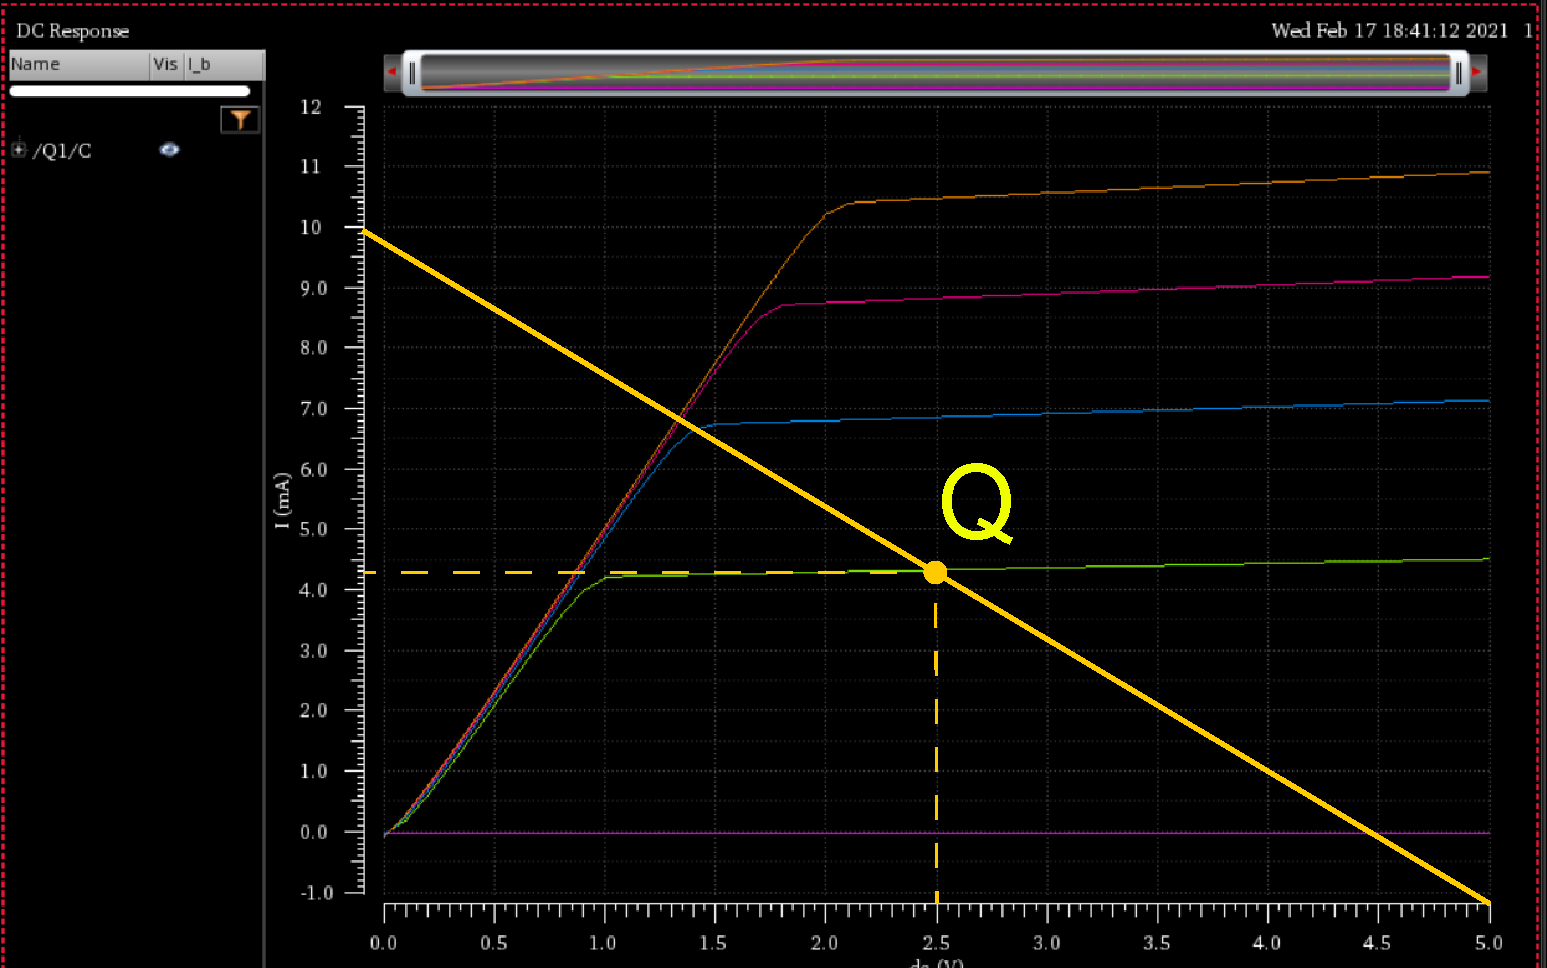
\includegraphics[height = 7 cm,width=18 cm]{1.png}
\end{center}

В донорном полупроводнике:
\begin{center}
$\sigma_n = e\cdot n \cdot \mu_n$\\
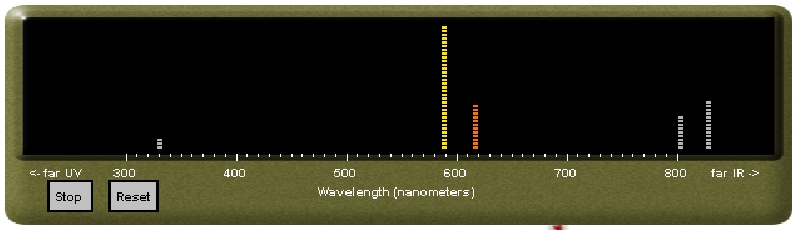
\includegraphics[height = 9 cm,width=18 cm]{3.png}
\end{center}

в случае преобладания акцепторных примесей:
\begin{center}
$\sigma_p = e\cdot p \cdot \mu_n$\\
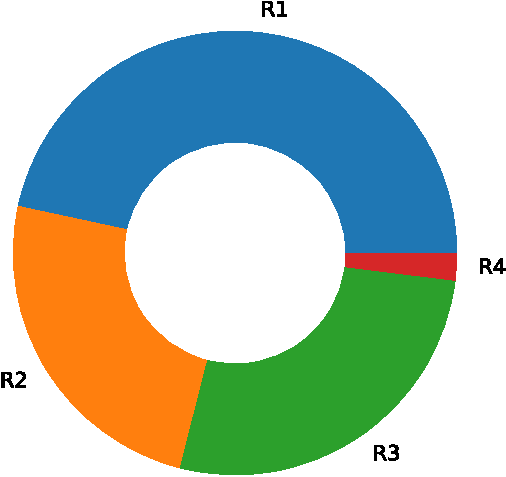
\includegraphics[height = 9 cm,width=18 cm]{2.png}\\
\end{center}

Рассмотрим поведение $\sigma$ полупроводника при переходе от низких температур к высоким. В донорном или акцепторном полупроводнике проводимость при низких температурах является примесной. Так как температура низкая, то ионизованных примесей мало и преобладает рассеяние на нейтральных атомах, при котором $\mu$ не меняется с температурой. Поэтому температурная зависимость $\sigma$ будет определяться зависимостью концентрации от температуры. Для электропроводности донорного полупроводника\\
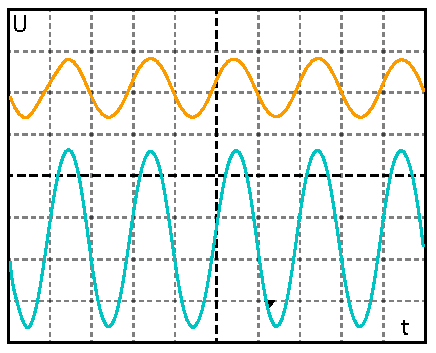
\includegraphics[height = 9 cm,width=18 cm]{4.png}\\



\end{document}